\chapter{MBZIRC challenge}\label{chap:thechallenge}
The Mohamed Bin Zayed International Robotics Challenge (MBZIRC) is an international robotics competition, held every two years \cite{challenge_description}. MBZIRC provides an ambitious and technologically demanding set of challenges, that aim to inspire the future of robotics through innovative solutions and technological excellence.\\
Robotics is poised to have a transformative impact in a variety of new markets and on various human social aspects. These include robot applications in disaster response, oil and gas, manufacturing, construction and household chores. Enabling technologies for such applications include robots working more autonomously in dynamic, unstructured environments, while collaborating and interacting with other robots and humans. \\
The competition consists in 3 challenges and this thesis consist in developing a framework to complete challenge number 1 that requires an UAV to land on a moving ground vehicle. 
The specifications of the challenge are:
\begin{itemize}
\item Duration: 20 minutes.
\item UAV initial condition: the participating team positions the UAV in stationary mode on the ground at the start location.
\item UGV initial condition: the ground vehicle is driven into the arena and placed at a random location on the track.
\end{itemize}

 

\subsection{The Arena}
The challenge will be performed in an arena with the following specifications (see figure \ref{fig:arenachallenge}):
\begin{itemize}
\item Outdoor open arena with GPS access.
\item Dimension: approximate  $100m \times 60m$.
\item Track: width 3m, in the shape of a figure 8 (of infinity shape), with boundary marked with white paint.
\item Terrain: relatively smooth and relatively level. 
\item UAV initial start location: 10m away from the arena.
\end{itemize}

\begin{figure}[!htbp]
    \centering
    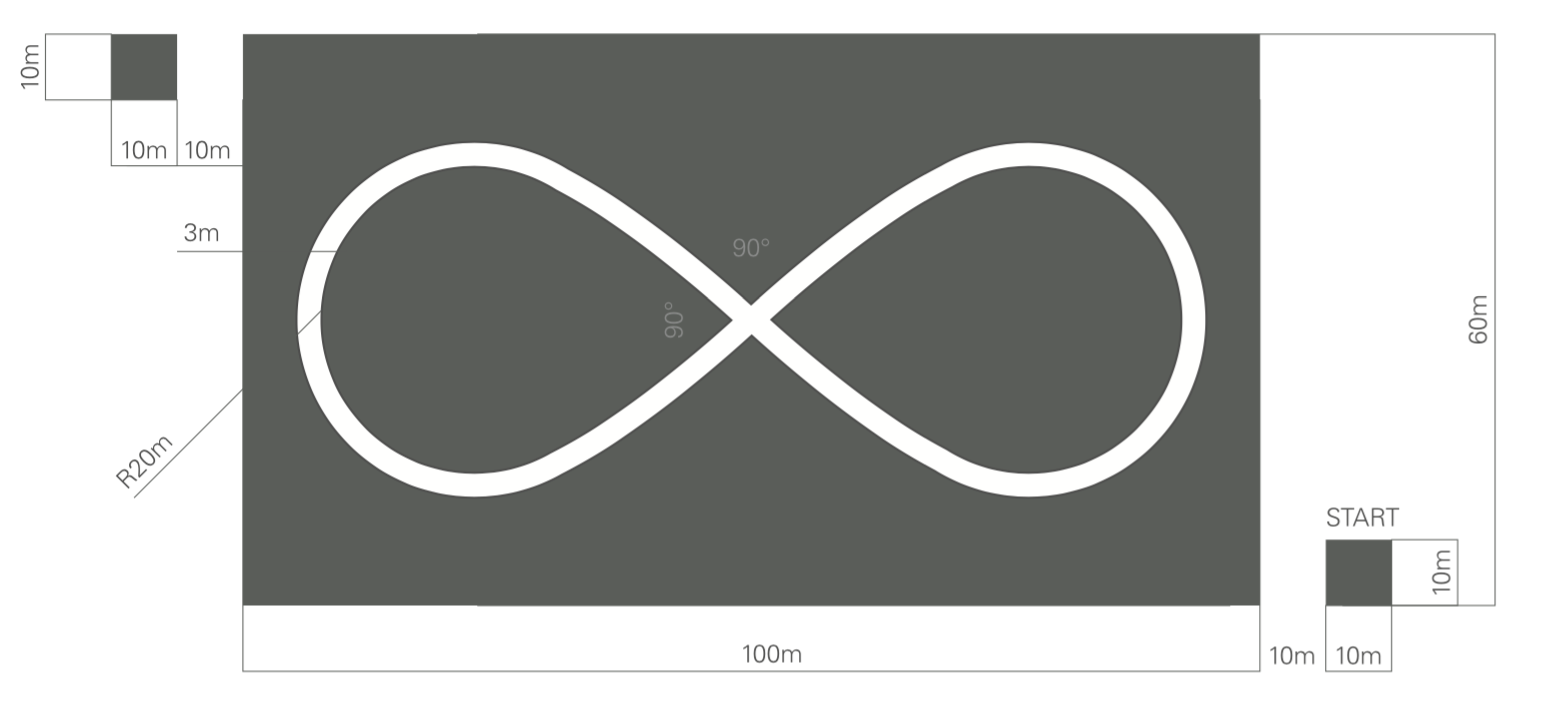
\includegraphics[width=1.1\textwidth]{img/arena.png}
    \caption{Arena of the challenge}
    \label{fig:arenachallenge}
\end{figure}

\subsection{Landing platform}
The landing platform is mounted on a ground vehicle of approximate dimensions $2.5m \times 1.5m \times 1.5m$ (length, width, height). The moving car starts at a constant speed of $15km/h$, it reduces the speed to $10km/h$ after 6 minutes and to $5 Km/h$ after 12 minutes.\\
The landing platform will be made of a ferrous surface to enable docking using magnetic or suction or other means.
It will be a square of dimensions $1.5m \times 1.5m$, and approximately $1.5m$ above ground, positioned on the vehicle. 
The landing zone inside the landing area is a circle of diameter $1m$. The center of the circle is indicated by an X. The landing area, the landing zone and the marker X are shown in Figure \ref{fig:finalplatform}.
A successful landing is when a point of contact of the UAV is within the landing circle, with propulsion off and rotors not spinning.

\begin{figure}[!htbp]
    \centering
    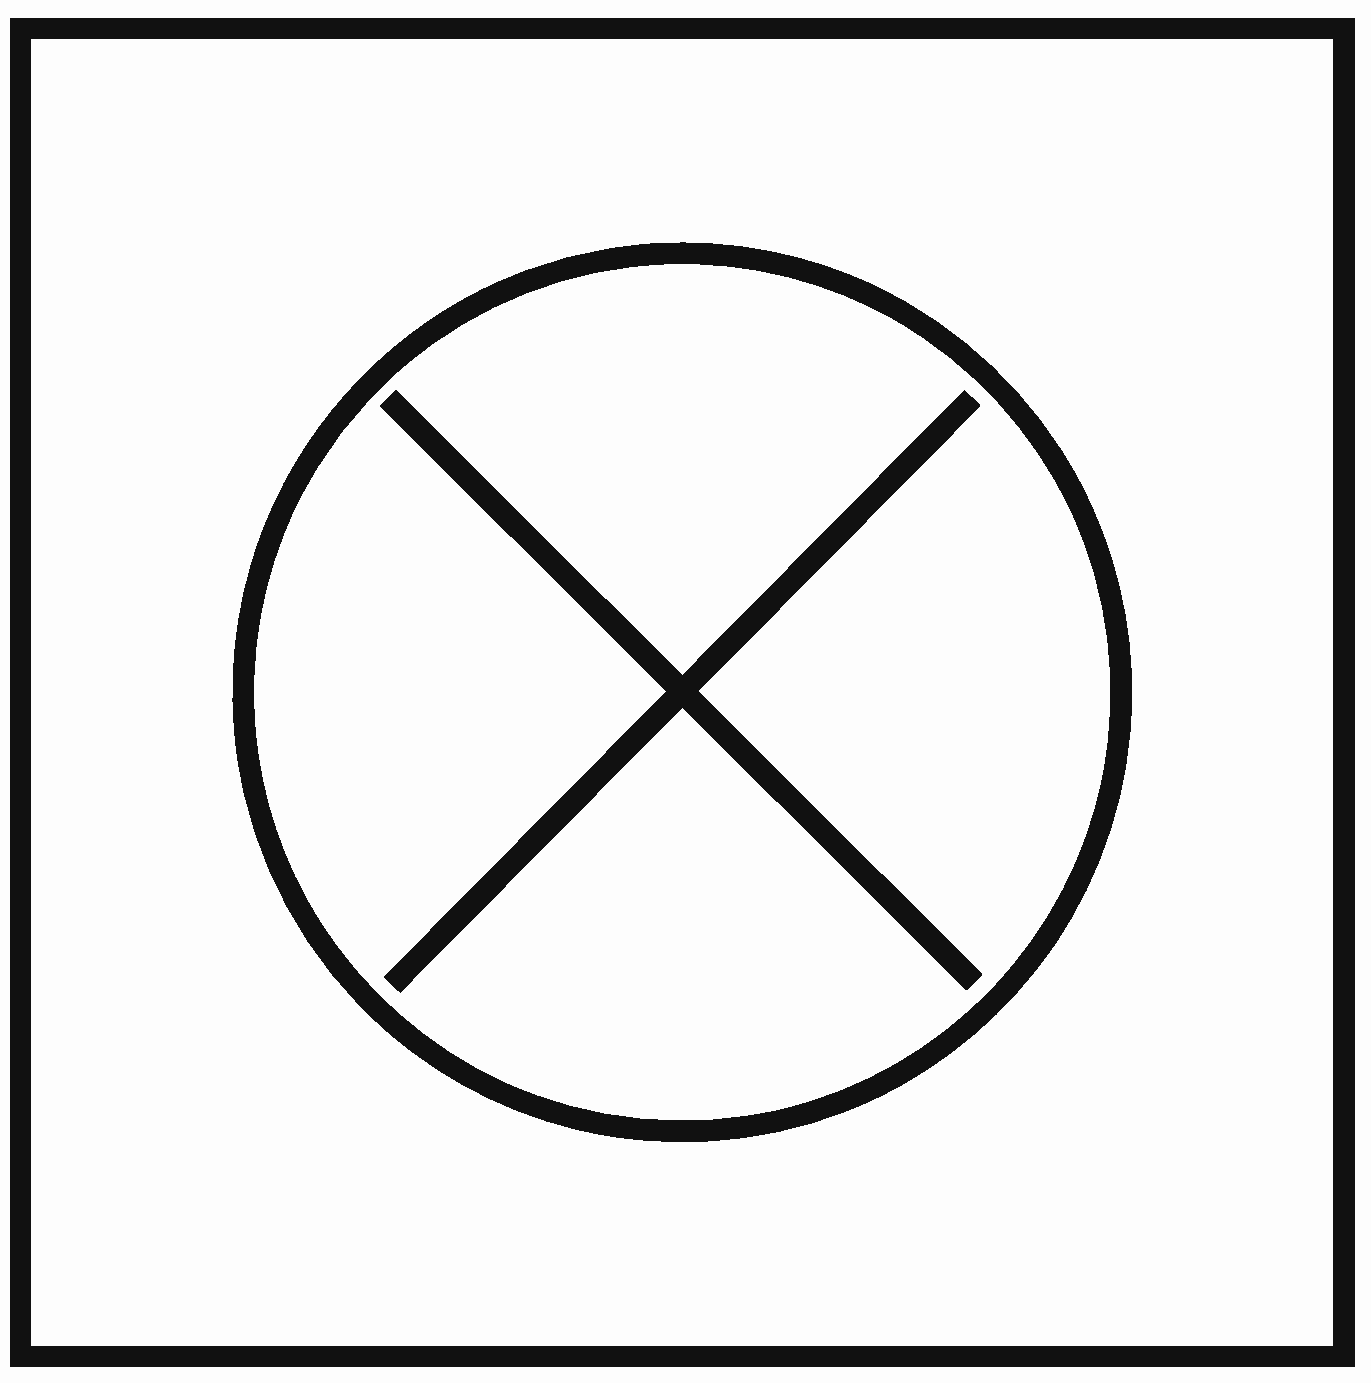
\includegraphics[width=0.5\textwidth]{img/base.pdf}
    \caption{Design of the platform in which the quadrotor must land on}
    \label{fig:finalplatform}
\end{figure}

\subsection{Infinity shape path}
The moving platform will move in an infinity-shape path described in the figure \ref{fig:arenachallenge}. 
We need to describe in a mathematical way this shape in order to use this information when we are estimating the state of the platform and to understand the right moment to perform the landing maneuver.\\
From the specification of the challenge:
\begin{itemize}
\item the car is moving with constant velocity $v_{tan}$ along the path
\item the radius of the circumferences that forms the trajectory is $r_{8}$m
\item the path is making a cross in the middle that creates 4 angles of $\frac{\pi}{2}$ 
\end{itemize}
The easiest way to describe this path is to define how the angle $\theta$ is changing in function of the space. \\
It easy to see that the shape can be seen as a combination of a cross and two circles.
The cross is simply defined as the union between the two line:
\begin{align}
\begin{split}
y &= x \\
y &= -x
\end{split}
\end{align}
while the two circles 
\begin{align}
\begin{split}
y^2 + (x - x_0)^2 &= r_{8}^2 \\
y^2 + (x + x_0)^2 &= r_{8}^2 
\end{split}
\end{align}
It easy to see that if we want the intersections between these two functions to be exactly in the 4 points we have to choose 
\begin{align}
\begin{split}
x_0 = \frac{\sqrt{2}}{2}r_{8}
\end{split}
\end{align}
That correspond to the 4 intersections coordinate
\begin{align}
\begin{split}
\Big(\frac{\sqrt{2}}{2}r_{8},\frac{\sqrt{2}}{2}r_{8}\Big);
\Big(\frac{\sqrt{2}}{2}r_{8},-\frac{\sqrt{2}}{2}r_{8}\Big);
\Big(-\frac{\sqrt{2}}{2}r_{8},-\frac{\sqrt{2}}{2}r_{8}\Big);
\Big(-\frac{\sqrt{2}}{2}r_{8},\frac{\sqrt{2}}{2}r_{8}\Big)
\end{split}
\end{align}

\begin{figure}[!htbp]
  \centering
 {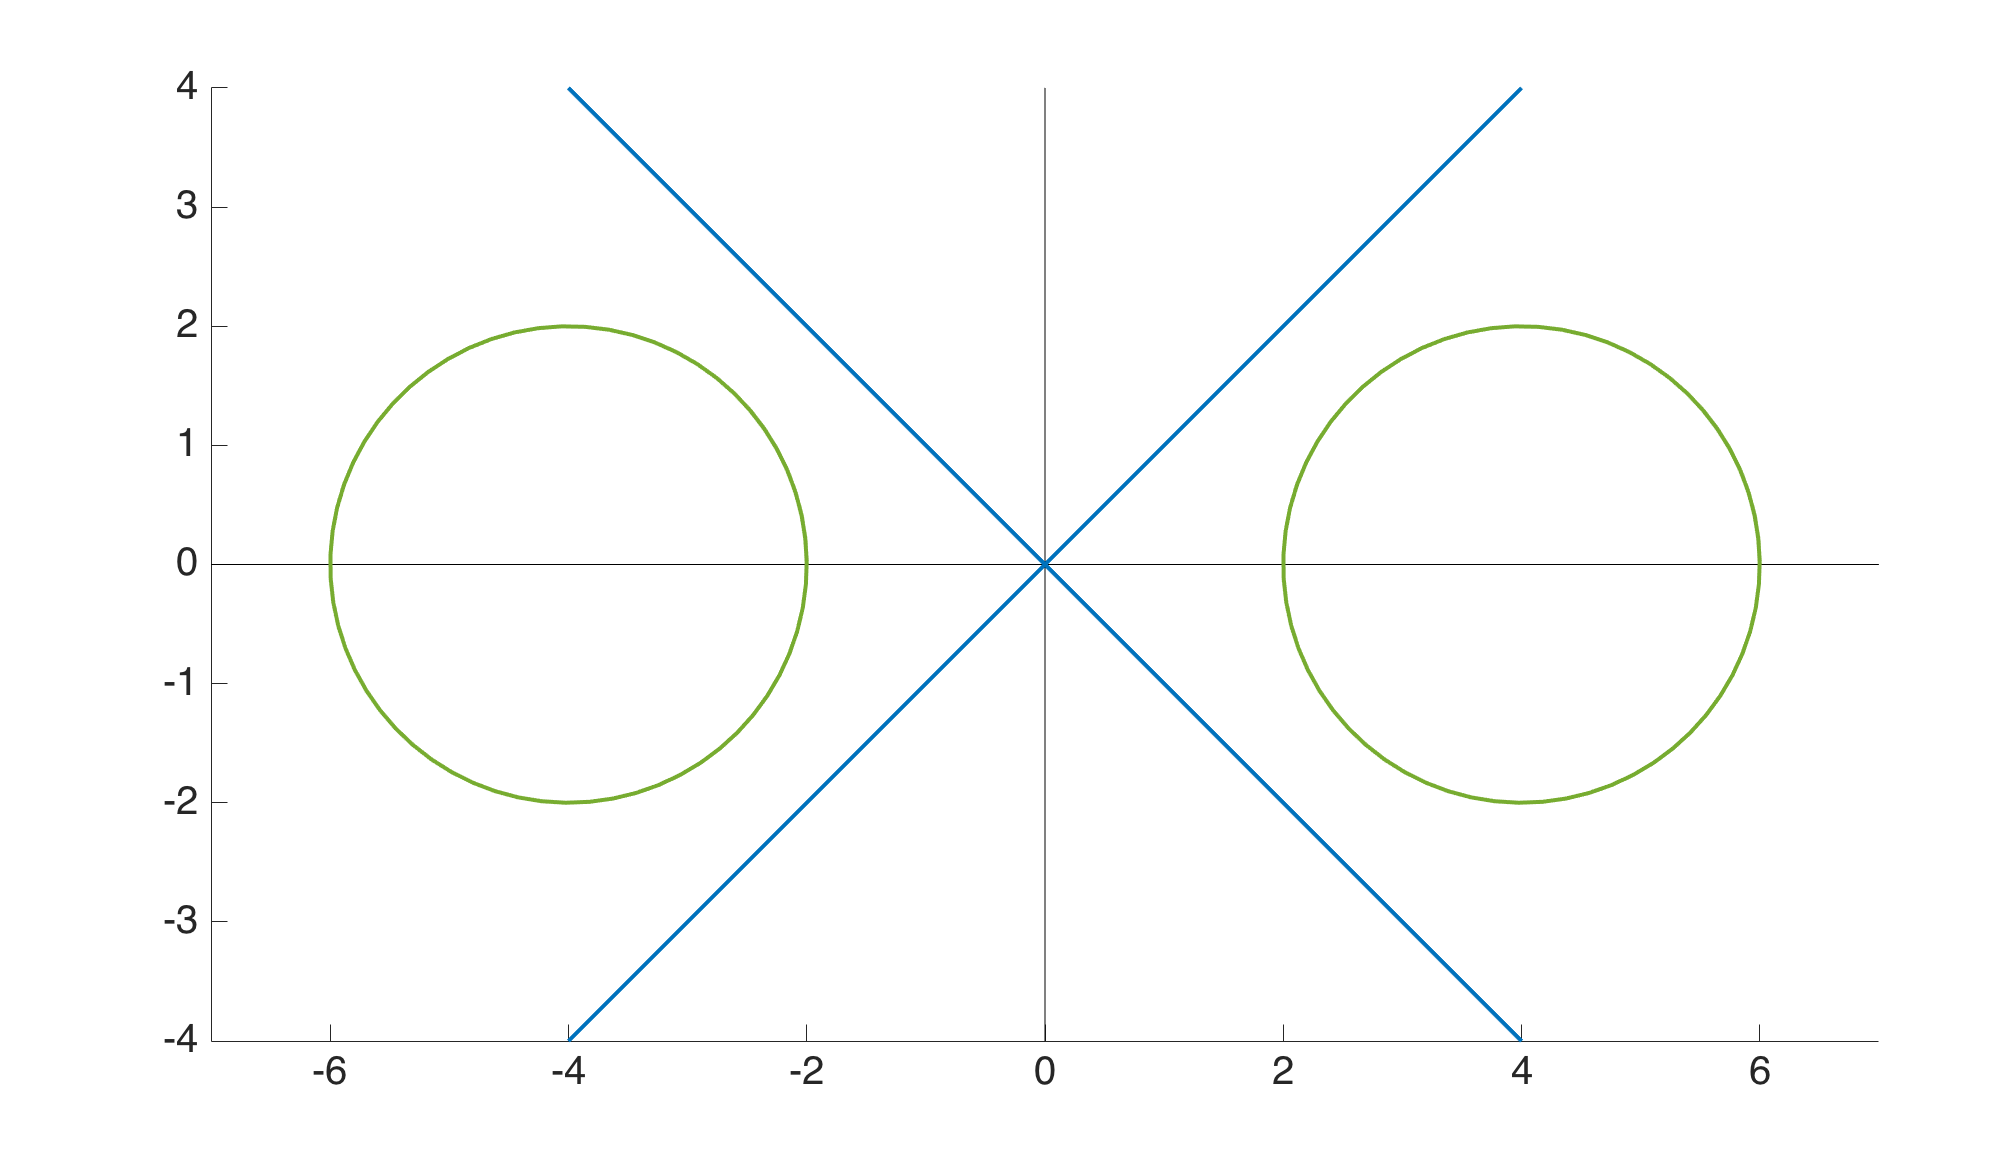
\includegraphics[width=0.48\textwidth]{img/constructionshape1_.png}\label{fig:constuctinfinity1}}
  \hfill
  {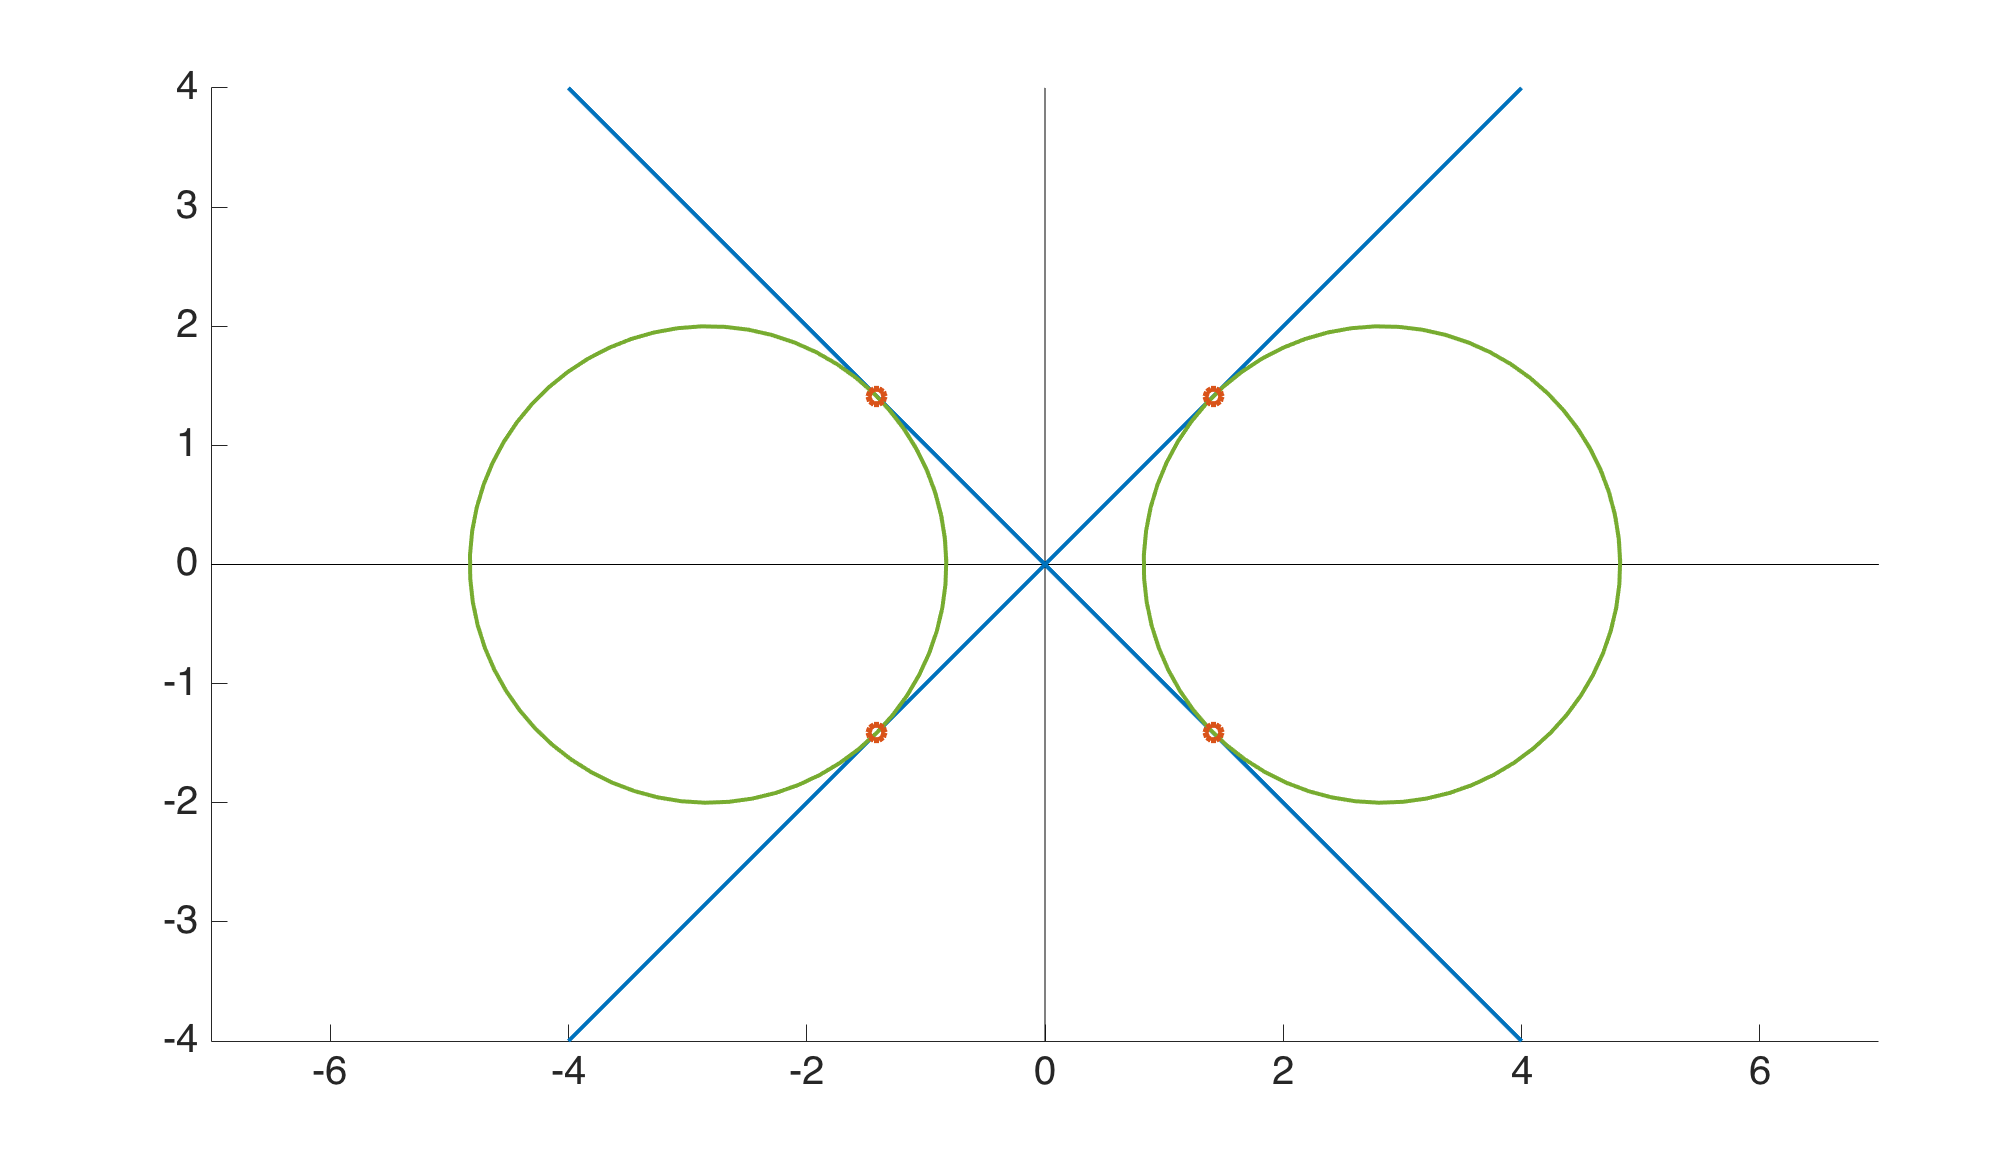
\includegraphics[width=0.48\textwidth]{img/constructionshape2_.png}\label{fig:constuctinfinity2}}
  \caption{How to construct the infinity-shape path}
\end{figure}

If we travel over the two circumferences the intersections correspond to angles $\theta = \pm \frac{3\pi}{4}$. \\
Now it is obvious to see that the path is symmetric and it can be divided in 4 parts and describing how the angle is changing in one of this section, the whole trajectory is defined.\\
We can observe that:
\begin{align}
\theta(x) =
\begin{cases}
    -\frac{x}{r_{8}}  &x\in \Big[0,\frac{3\pi}{4}r_{8}\Big] \quad \quad \ \ \  \\[10pt]
    -\frac{3\pi}{4} &x\in \Big[\frac{3\pi}{4}r_{8} ,\frac{3\pi}{4}r_{8} + r_{8}\Big]
\end{cases}
\end{align}
This function define a quarter of the trajectory \ref{fig:quarter_path} in function of the radius $r_{8}$ of the path.\\
It is now possible to use it to generate the entire trajectory $( x(t) , y(t) )$ \ref{fig:entire_path}: \\ we know that the length of the path is $$l = 4(\frac{3\pi}{4}r_{8} + r_{8})$$
and given the constant velocity $v_{tan}$ we can calculate the time to complete the trajectory 
$$T = \frac{l}{v_{tan}}$$
and it is simple to define $\theta(t)$ just stretching or shrinking $\theta(x)$ .\\
So we can now define:
\begin{align}
\begin{split}
\dot{x} &= v_{tan} cos(\theta(t)) \\
\dot{y} &= v_{tan} sin(\theta(t))
\end{split}
\end{align}
And finally we also need the discretized verison obtain just by forward Euler approximation:
\begin{align}
\begin{split}
x_k &= x_{k-1} + dt \big(v_{tan k-1} cos(\theta_{k-1})\big) \\
y_k &= y_{k-1} + dt \big(v_{tan k-1} sin(\theta_{k-1})\big)
\end{split}
\end{align}

\begin{figure}[!htbp]
  \centering
 {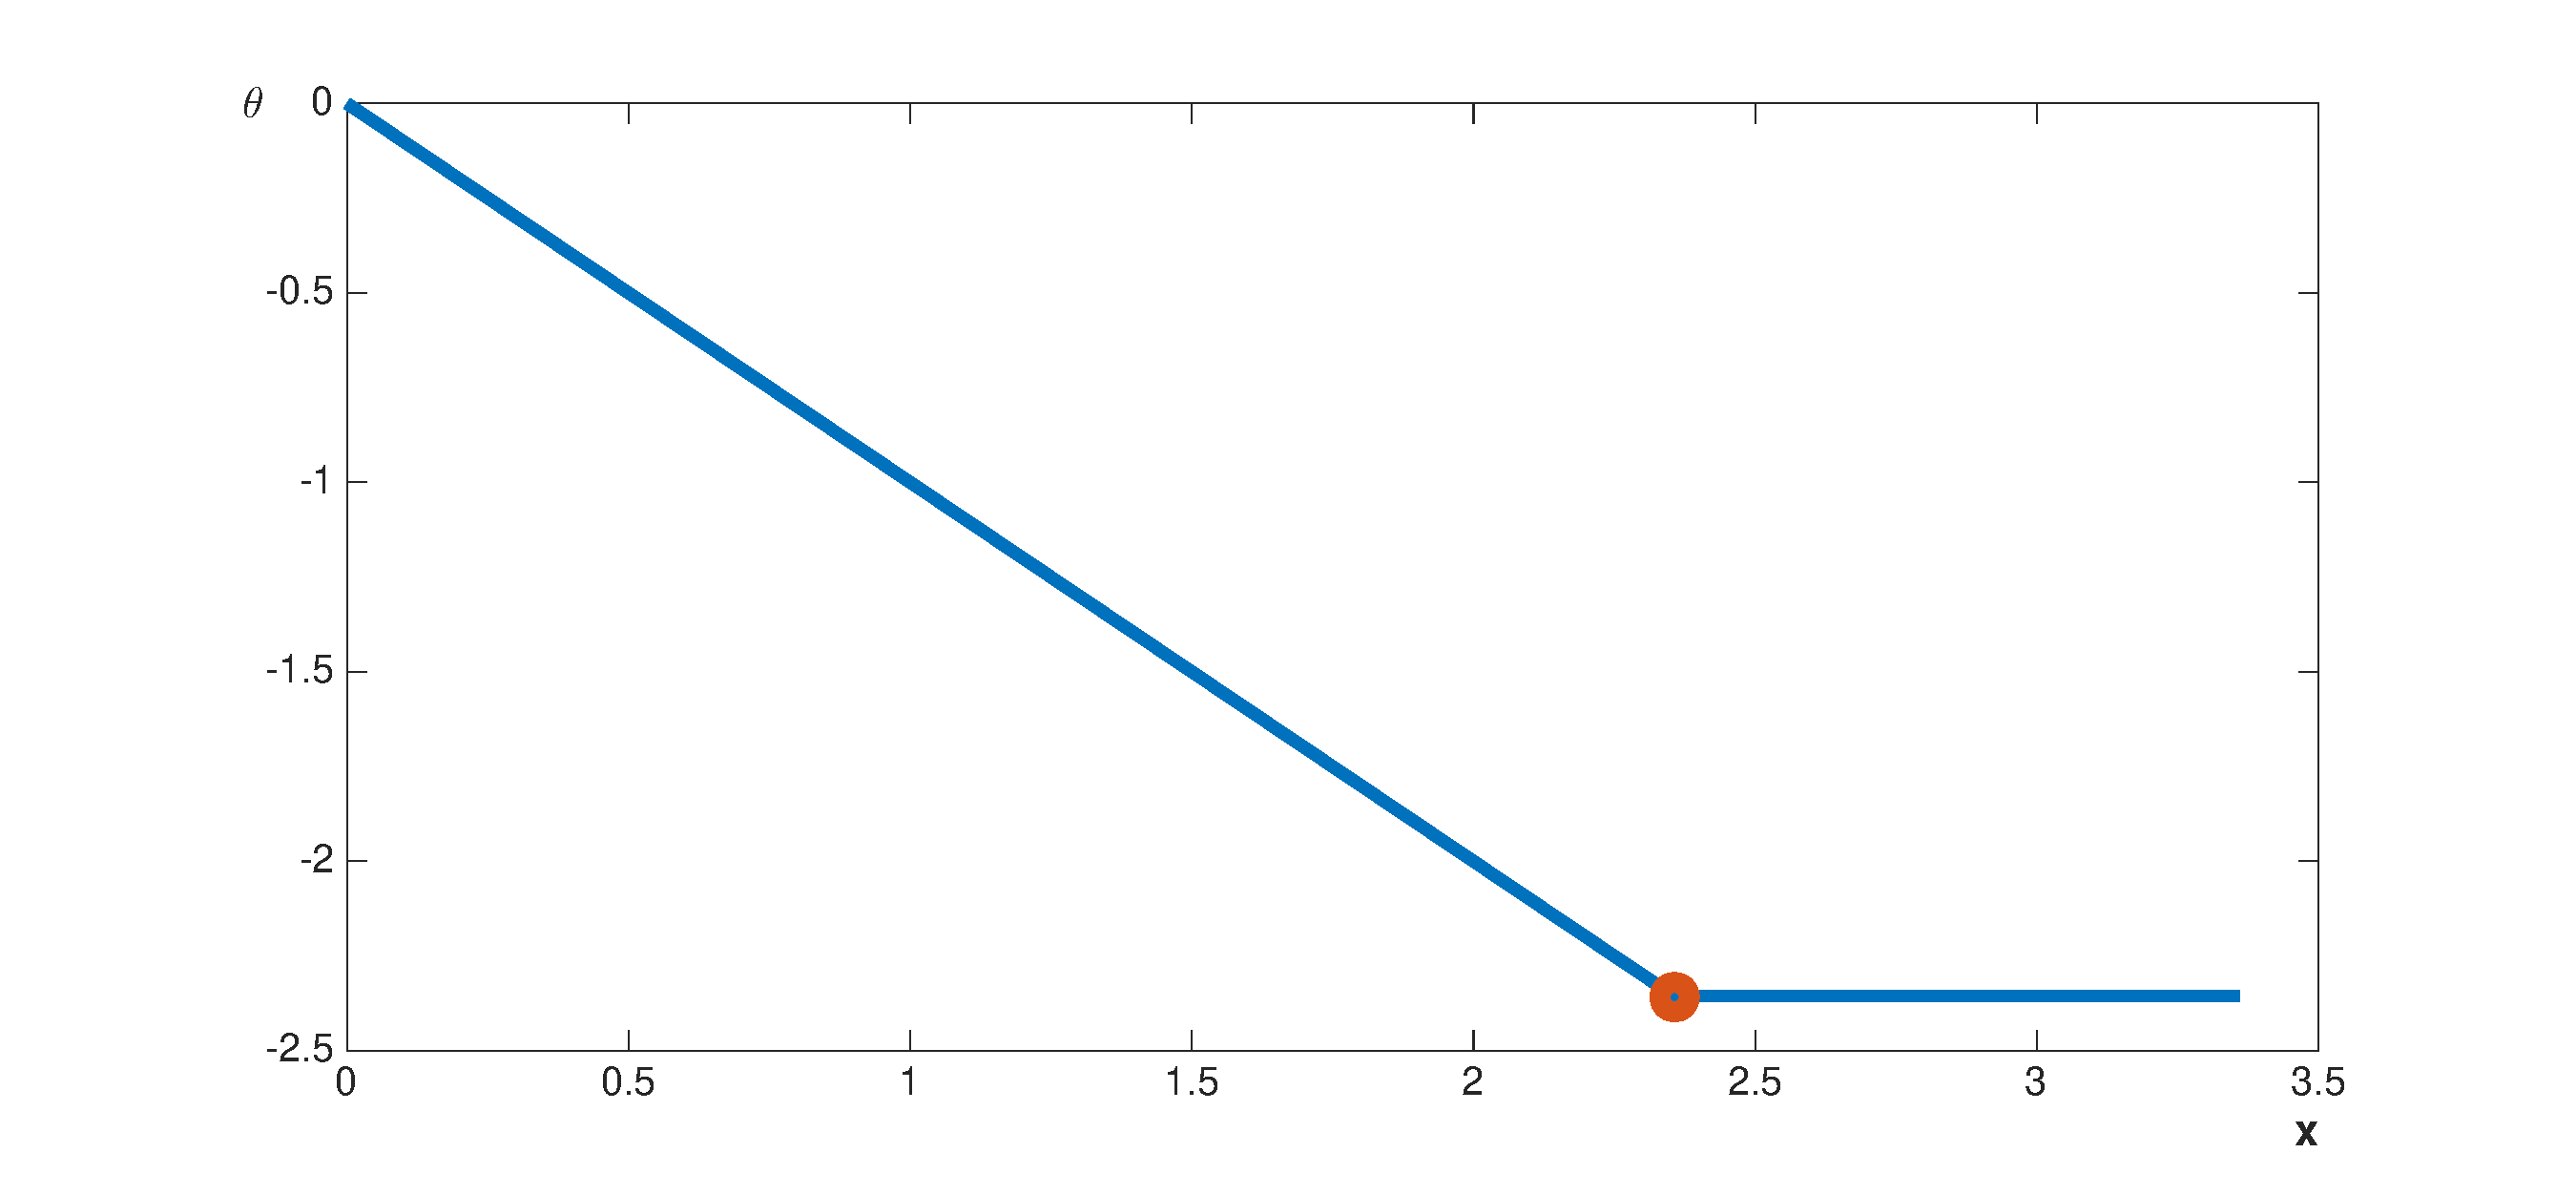
\includegraphics[width=0.8\textwidth]{img/angle_x.eps}\label{fig:quarter_theta}}
  \hfill
  {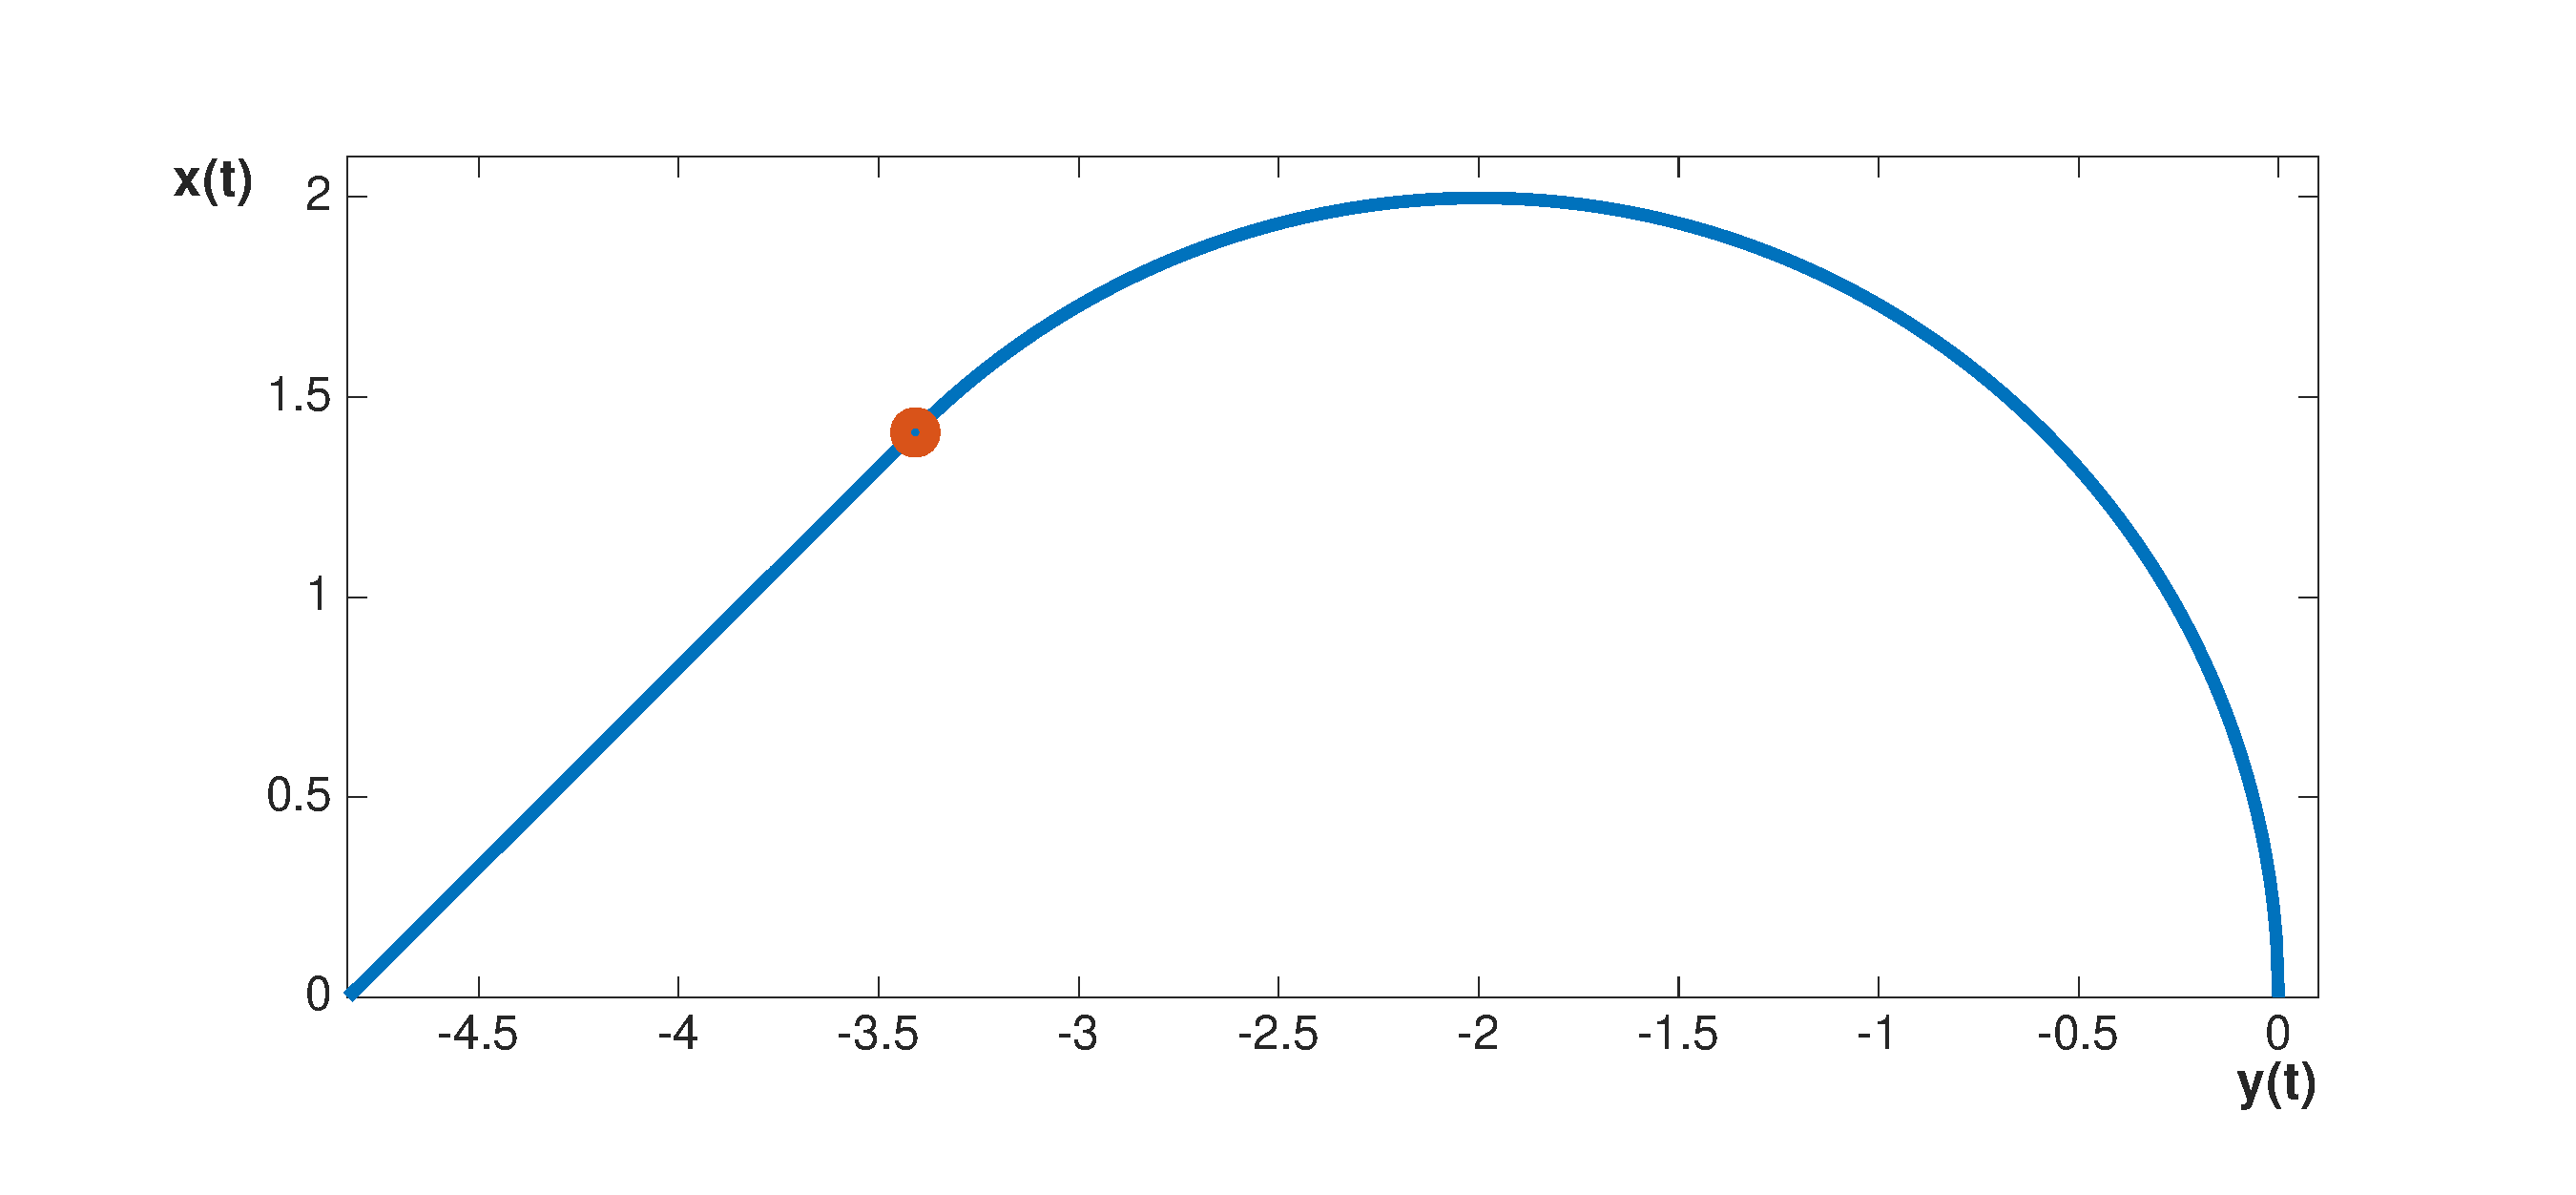
\includegraphics[width=0.8\textwidth]{img/path_x_quarter.eps}\label{fig:quarter_xy}}
  \caption{The parametrization of a quarter of the path}
  \label{fig:quarter_path}
\end{figure}

\begin{figure}[!htbp]
    \centering
    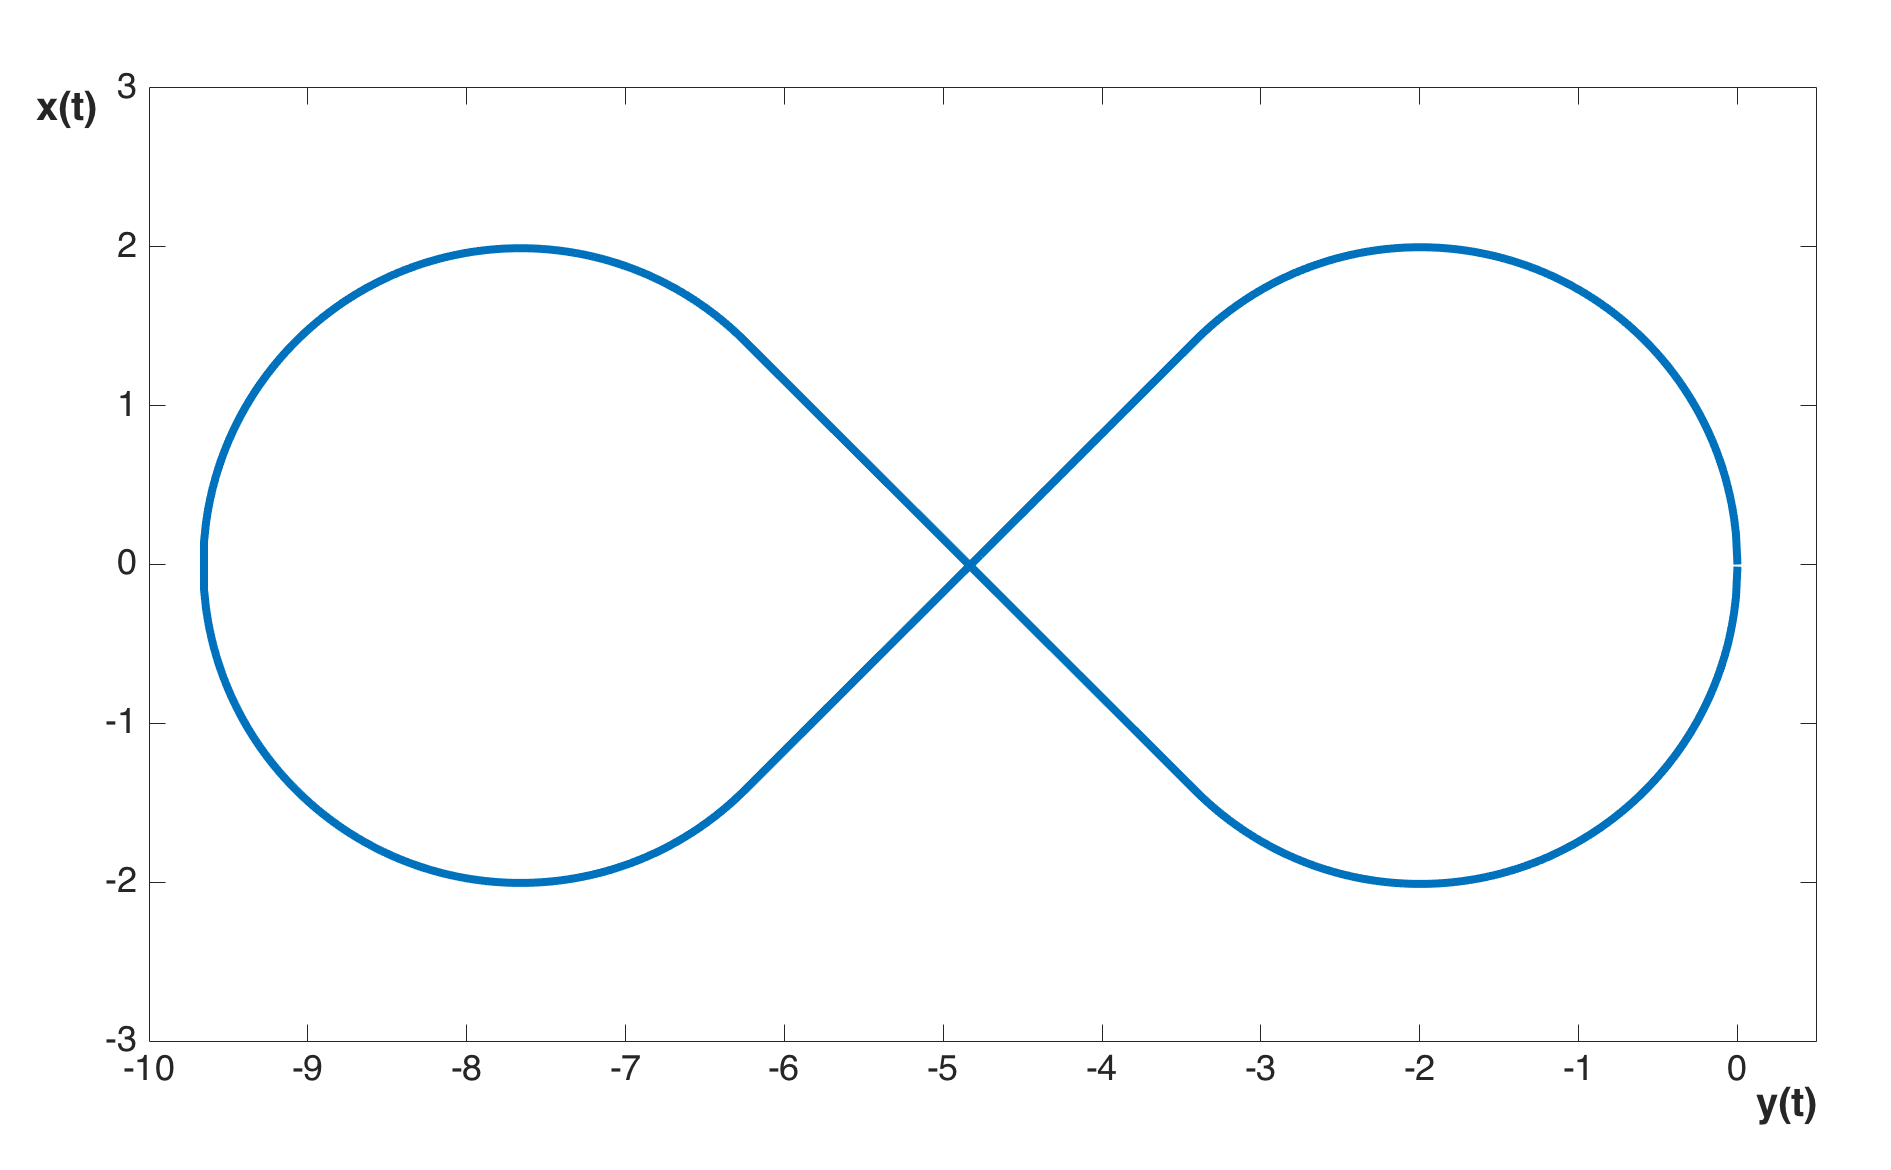
\includegraphics[width=1\textwidth]{img/infinityshapepath.png}
    \caption{Infinity-shape path}
    \label{fig:entire_path}
\end{figure}

\section{Simulation}

